%!TEX root = Report.tex

\subsection{Tracking}
\label{tracking}
As mentioned in the project proposal the project was divided into three parts. The first part of the project was to be able to track termites. Since african termites are hard to come by and transport we settled for giant ants (Camponotus Ligniperdus), which are the largest ants found in Denmark \cite{fogn}, instead. While these are not as big as the termites, they behave in a similar way and the solution should be able to easily adapt to the termites. In the first part we started by implementing the tracking on a video. We received a video from Harvard of a single ant running around in a petri dish with a white background. The ant itself was painted red and green to make tracking easier. This was the simplest setup we could think of and acted as a good starting point. By recommendation we decided to use the OpenCV \cite{opencv} framework to implement our tracking. We will return to this framework in Section \ref{framework} Framework. \\

This chapter is divided into three subparts. First we will introduce the reader to different image processesing techniques, and their uses. Following this we will introduce the reader to a framework that supports these techniques, and finish off describing the implemented solution and design choices.

% Gå ud fra at dette afsnit ikke har noget video input fra et kamera. Integration med kameraet kommer senere.
% 
% Teori først - hvilken slags image manipulation har vi brugt? hvad var alternativerne?
% Så framework - vi bruger OpenCV, why? hvad giver det os? hvad er drawbacks?
% så implementation - Hvad har vi implementeret? Hvordan var performance? hvad var vores alternativer? har vi eksperiementeret med nogen af de andre muligheder?
% 
% Image Segmentation - hvad giver det os/hvorfor er det smart?
% Thresholding
% Dilating
% Eroding
% Background detection and why we can't use it
% Alternatives and why we don't use them

\subsubsection{Theory} \mbox{}\par
\todo{Rewrite chapter a bit - make it self contained. Keep writing WHY this is important and interesting to read and how it will help track ants.}
This section will provide information about five common image processing techniques; thresholding, dilating and eroding, contrast, image segmentation and background filtering. The description of each technique will be backed up by examples. We will also use the \textit{ternary if} statement notation in this section which looks like the one shown in Equation \ref{eq:notation}.

\begin{equation}
value = {Boolean\mbox{-}Condition} ? {True\mbox{-}Evaluation}: {False\mbox{-}Evaluation}
\label{eq:notation}
\end{equation}

It works just like you would expect from many programming languages. It is also known as an inline \textit{if-statement}. \\

\noindent \textbf{Thresholding} \par
Thresholding is an image processing technique used to make a final decision about each pixel in an image. Either a pixel value is one that we are interested in or it is not. This is usually done by assigning a specific pixel value to the pixel we want, and another to those that we do not want. In general we compare the \textit{i}th pixel of the source image, \textit{src}, to the threshold value, \textit{T}, and saves the result in a destination image, \textit{dst}. For instance, to create a binary image where we are interested in all pixels above the threshold \textit{T}, the equation would look like the one shown in Equation \ref{eq:binarythresholding},

\begin{equation}
dst_i = src_i \geq T ? 255: 0
\label{eq:binarythresholding}
\end{equation}

Most threshold operations are applied on grayscale images, where all pixel values range between 0 (black) and 255 (white). Sometimes these values are normalized to range between 0 and 1 instead. However for the rest of this report we will assume that grayscale images use the former convention. Soon we will argue how thresholding can be expanded to also cover thresholding an RGB image. Figure \ref{fig:threshold_example} show an example of applying threshold to a grayscale image.

\begin{figure}
        \centering
        \begin{subfigure}[b]{0.3\textwidth}
                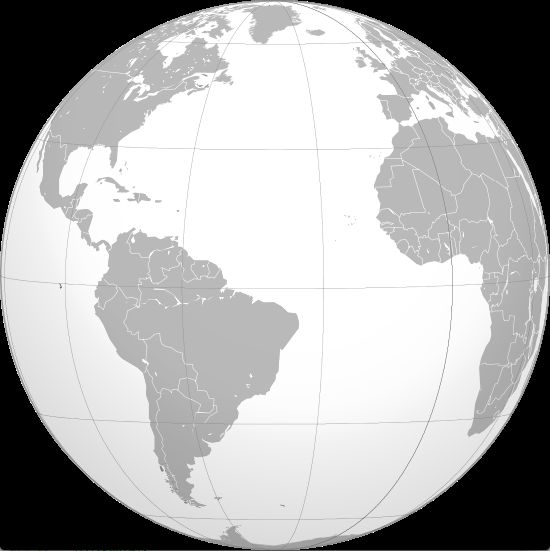
\includegraphics[scale = 0.2]{img/globe}
                \caption{Grayscale image}
        \end{subfigure}
		\quad
        \begin{subfigure}[b]{0.3\textwidth}
                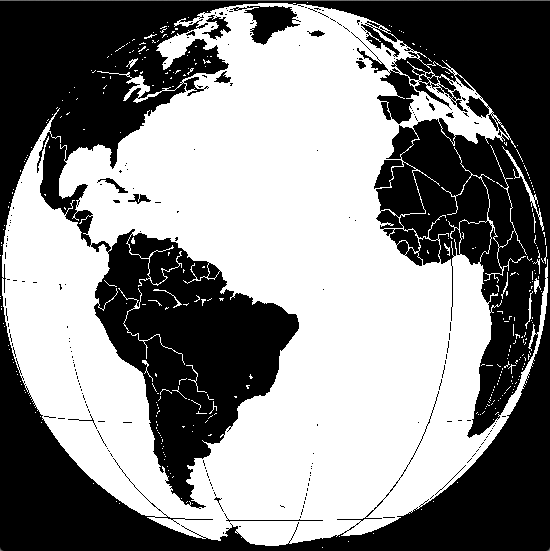
\includegraphics[scale = 0.2]{img/post_threshold}
                \caption{Thresholded image}
        \end{subfigure}
		\caption{An example of applying a threshold on a grayscale image. This example use the threshold value \textit{T} = 200}
		\label{fig:threshold_example}
\end{figure}

Now what happens if what you are interested in is a color? To use standard thresholding we first need to convert it to a grayscale image. However doing so might result in an image that have lost important information as can be seen in figure \ref{fig:RGB2GRAY}. Unless you want to find the red color, you have no way of differentiating the blue and green color.

\begin{figure}
        \centering
        \begin{subfigure}[b]{0.3\textwidth}
                
\includegraphics[scale=0.5]{img/RGB}
                \caption{RGB image}
        \end{subfigure}
		\quad
        \begin{subfigure}[b]{0.3\textwidth}
                
\includegraphics[scale=0.5]{img/GrayRGB}
                \caption{Grayscale image}
        \end{subfigure}
		\caption{Example of grayscaling a color image}
		\label{fig:RGB2GRAY}
\end{figure}

A step in the right direction would be to define the threshold value \textit{T} as a scalar consisting of three values - one for each color channel. We will denote this threshold scalar as \textit{S} and define it as shown in Equation \ref{eq:thresholdscalar}.

\begin{equation}
S =  
\begin{pmatrix}
  S_{R}\\
  S_{G}\\
  S_{B}\\
\end{pmatrix}
\label{eq:thresholdscalar}
\end{equation}

To apply it to an RGB image we need to change Equation \ref{eq:binarythresholding} to the one shown in Equation \ref{eq:threshold_RGB}.

\begin{equation}
{dst_i} = {src_i}_R \geq S_R \wedge {src_i}_G \geq S_G \wedge {src_i}_B \geq S_B? 255: 0
\label{eq:threshold_RGB}
\end{equation}

Trying it out makes it much easier to differentiate between colors. In Figure \ref{fig:RGB_Thresh} a threshold attemp using this method directly on the RGB image is shown.

\begin{figure}
        \centering
        \begin{subfigure}[b]{0.3\textwidth}
                
\includegraphics[scale=0.5]{img/RGB}
                \caption{RGB image}
        \end{subfigure}
		\quad
        \begin{subfigure}[b]{0.3\textwidth}
                
\includegraphics[scale=0.5]{img/RGBThresh}
                \caption{Thresholded image}
        \end{subfigure}
		\caption{Example of thresholding a color image with Equation \ref{eq:threshold_RGB} using the scalar \textit{S}=(0,100,0)}
		\label{fig:RGB_Thresh}
\end{figure}

However one issue remains - what if you want to find a color among similar colors? The problem is illustrated in Figure \ref{fig:green_fail} using the same scalar as in Figure \ref{fig:RGB_Thresh}

\begin{figure}
        \centering
        \begin{subfigure}[b]{0.3\textwidth}
                
\includegraphics[scale=0.5]{img/green}
                \caption{RGB image}
        \end{subfigure}
		\quad
        \begin{subfigure}[b]{0.3\textwidth}
                
\includegraphics[scale=0.5]{img/simpleRGBThresh}
                \caption{Thresholded image}
        \end{subfigure}
		\caption{Example of thresholding a color image with Equation \ref{eq:threshold_RGB} using the scalar \textit{S}=(0,100,0). Unlike before the result is unsatisfactory.}
		\label{fig:green_fail}
\end{figure}

The solution is to specify a \textit{range} of acceptable values instead of just a threshold. We will specify two scalars; S Upper, \textit{SU}, and S Lower, \textit{SL}.

\begin{equation}
SL =  
\begin{pmatrix}
  SL_{R}\\
  SL_{G}\\
  SL_{B}\\
\end{pmatrix}
\label{eq:thresholdlower}
\end{equation}

\begin{equation}
SU =  
\begin{pmatrix}
  SU_{R}\\
  SU_{G}\\
  SU_{B}\\
\end{pmatrix}
\label{eq:thresholdupper}
\end{equation}

We will use the definitions in Equations \ref{eq:thresholdlower} and \ref{eq:thresholdupper} to update Equation \ref{eq:threshold_RGB}. The changes can be seen in Equation \ref{eq:threshold_range}.

\begin{equation}
{dst_i} = SU_R \geq {src_i}_R \geq SL_R \wedge SU_G \geq {src_i}_G \geq SL_G \wedge SU_B \geq {src_i}_B \geq SL_B? 255: 0
\label{eq:threshold_range}
\end{equation}

Using a range to specify a color instead will yield a much more satisfactory result as shown in Figure \ref{fig:green_final}. \\

\begin{figure}
        \centering
        \begin{subfigure}[b]{0.3\textwidth}
                
\includegraphics[scale=0.5]{img/green}
                \caption{RGB image}
        \end{subfigure}
		\quad
        \begin{subfigure}[b]{0.3\textwidth}
                
\includegraphics[scale=0.5]{img/finalthresh}
                \caption{Thresholded image}
        \end{subfigure}
		\caption{Example of thresholding a color image with Equation \ref{eq:threshold_range} using the range \textit{SL}=(0,100,0) and \textit{SU}=(1,150,10). We have sucessfully located the dark green color area.}
		\label{fig:green_final}
\end{figure}

\newpage

\noindent \textbf{Dilation and Erosion} \par
% Forklar at vi har en kernel, B, med størrelsen s, der bliver anvendt på hver pixel, p, i et billede A.
% Angiv at dilating finder local optima, og at eroding finder local minima.
% Angiv at de her metoder bliver brugt EFTER thresholding for at "rense" billedet. \\

The basic concepts of \textit{morphological transformations} are \textit{dilation} and \textit{erosion}. These concepts are mostly used to remove noice, isolating individual elements or joining disparate elements in an image. These transformations are applied to either grayscale or binary image, and are often used to clean up an image after thresholding to make analysing the image easier. The way both erosion and dilation are applied to an image is by defining a kernel, denoted \textit{B}, that will be applied to an image (or part of an image), denoted \textit{A}. The kernel can be any shape or size, however it is often a square where the sides are uneven, e.g. 3x3, 5x5, 7x7 and so on. A kernel has an \textit{anchorpoint}, which is the pixel in A that erosion or dilation are applied on, and the result is stored in the corresponding point in the destination image, \textit{dst(i.j)}. Figure \ref{fig:kernel_ed} shows an example of a kernel and its anchorpoint in the center. \\

\begin{figure}[ht!]
  \centering
    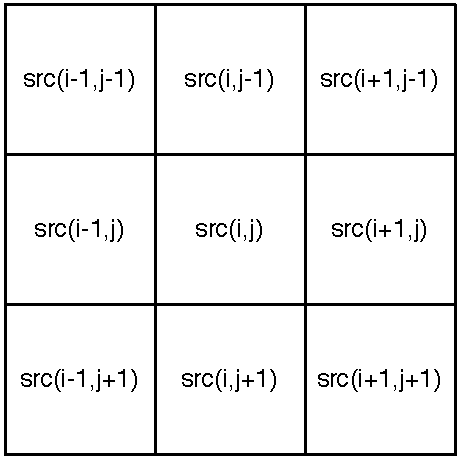
\includegraphics[scale=0.50]{img/Kernel_ED.pdf}
  \caption{Given a pixel, src(i.j) the kernel covers the neighbouring pixels. Shown here is a 3x3 kernel.}
  \label{fig:kernel_ed}
\end{figure}

When transforming an image using dilation, whenever the kernel is applied to a new anchorpoint, the \textit{local optima} is used. When eroding an image the \textit{local minima} is used. Naturally, compared to the original image, bright areas are expanded when dilating, and dark areas are expanded when eroding. However one cannot say that e.g. eroding removes noice and dilating does not. It depends on the image which the transformation is applied on. Figure \ref{fig:sample_kernel} shows an example of pixels used to determine the outcome of the anchorpoint in the destination image. \\

\begin{figure}[ht!]
  \centering
    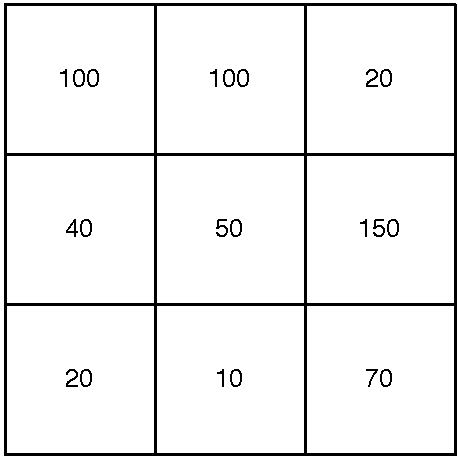
\includegraphics[scale=0.50]{img/sample_kernel.pdf}
  \caption{An example of a kernel within a source image, src. The value assigned to the destination image, dst(i,j), is 10 if erosion is chosen, else 150 if dilation is chosen.}
  \label{fig:sample_kernel}
\end{figure}

An example of how this applies to a real image is shown in Figure \ref{fig:erodedilate}. It is clear from this example how differently erosion and dilation affects an image.\\

\begin{figure}[!ht]
        \centering
        \begin{subfigure}[b]{0.3\textwidth}
                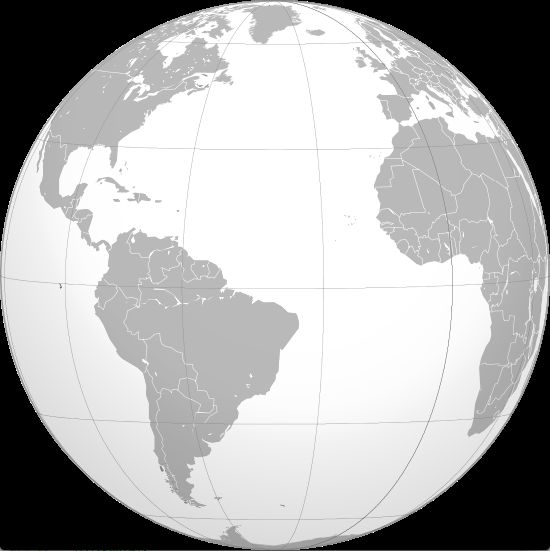
\includegraphics[scale = 0.2]{img/globe}
                \caption{Grayscale image}
        \end{subfigure}
		\quad
        \begin{subfigure}[b]{0.3\textwidth}
                
\includegraphics[scale = 0.2]{img/erode}
                \caption{Eroded image}
        \end{subfigure}
		\quad
        \begin{subfigure}[b]{0.3\textwidth}
                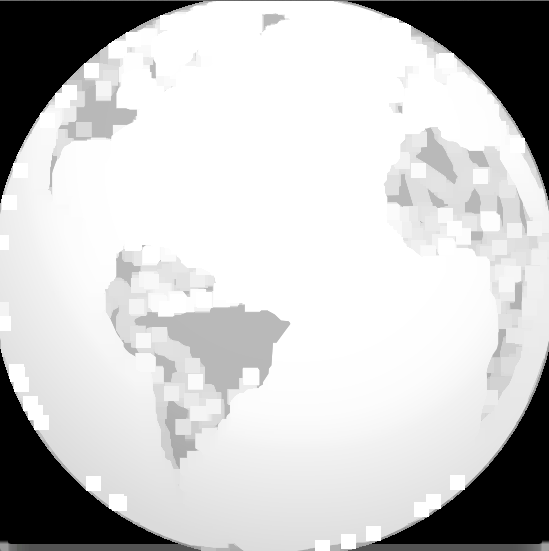
\includegraphics[scale = 0.2]{img/dilate}
                \caption{Dilated image}
        \end{subfigure}
		\caption{Eroding and dilating an image. It is clear that eroding expands dark areas and dilate expands bright areas. This example uses a 7x7 kernel.}
		\label{fig:erodedilate}
\end{figure}

Unlike thresholding we cannot apply erosion or dilation to RGB images due to the nature of \textit{RGB} values. Imagine the clear colors, red (255,0,0), green (0,255,0) and blue(0,0,255) - how can we argue which color is \textit{greater} or \textit{smaller} than the other? We cannot. We can with grayscale and binary images since we can safely say that the pixel value 150 is smaller than 255, and 0 is smaller than 1. We cannot for color images. \\

\noindent \textbf{Contrast and Brightness} \par
Where dilation and erosion sought to expand either dark or bright areas, contrast and brightness seek to increase the overall brightness or darkness of an image or the absolute difference between dark and bright pixels. To increase the absolute difference difference between two pixels, or \textit{increasing the contrast of the image}, each pixel in an image is multiplied with the same scalar, denoted $\alpha$. Since images are basically matrices this method is equal to \textit{scalar multiplication} shown in Equation \ref{eq:matrix_mul}.

\begin{equation}
\alpha \times 
\setlength{\arraycolsep}{5pt}
 \begin{bmatrix}
  a & b & c \\
  d & e & f \\
  g & h & i \\
 \end{bmatrix} =
 \setlength{\arraycolsep}{5pt} 
 \begin{bmatrix}
  \alpha \times a & \alpha \times b & \alpha \times c \\
  \alpha \times d & \alpha \times e & \alpha \times f \\
  \alpha \times g & \alpha \times h & \alpha \times i \\
 \end{bmatrix}
 \label{eq:matrix_mul}
\end{equation}

To increase the brightness each pixel is added with a scalar, denoted $\beta$ instead. This way the absolute difference between each pixel is kept, however all pixels get darker or brighter depending on the scalar. Similar to contrast this operation is equal to \textit{scalar addition} as shown in Equation \ref{eq:matrix_add}. To make the pixels brighter a positive scalar is used, to make it darker a negative scalar is used. Figure \ref{fig:bright_contrast} shows the result of contrasting and increasing the brightness of an image. Contrast and brightness are used to make dark, bright and diffuse images easier to analyse. \\

\begin{equation}
\beta + 
\setlength{\arraycolsep}{5pt}
 \begin{bmatrix}
  a & b & c \\
  d & e & f \\
  g & h & i \\
 \end{bmatrix} =
 \setlength{\arraycolsep}{5pt} 
 \begin{bmatrix}
  \beta + a & \beta + b & \beta + c \\
  \beta + d & \beta + e & \beta + f \\
  \beta + g & \beta + h & \beta + i \\
 \end{bmatrix}
 \label{eq:matrix_add}
\end{equation}

\begin{figure}
        \centering
        \begin{subfigure}[b]{0.3\textwidth}
                
\includegraphics[scale = 0.2]{img/colorGlobe}
                \caption{Source image}
        \end{subfigure}
		\quad
        \begin{subfigure}[b]{0.3\textwidth}
                
\includegraphics[scale = 0.2]{img/globeBright}
                \caption{Brightened image}
        \end{subfigure}
        \begin{subfigure}[b]{0.3\textwidth}
                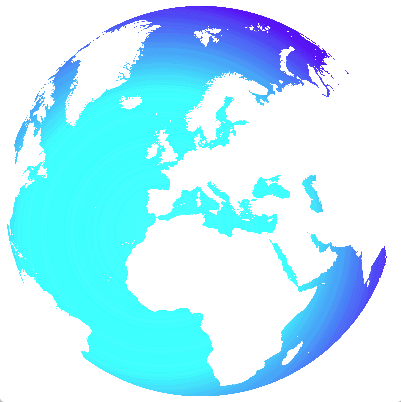
\includegraphics[scale = 0.2]{img/globeContrast}
                \caption{Contrasted image}
        \end{subfigure}
		\caption{Example of increasing the contrast and brigtness of an image. For this example $\alpha = 5$ and $\beta = 100$}
		\label{fig:bright_contrast}
\end{figure}

\noindent \textbf{Image Segmentation} \par
Image segmentation is the processing of partitioning all the pixels in an image into \textit{S} segments (or superpixels). The goal is to simplify an or change the representation of an image such that it is easier to analyse. It is mostly used to locate objects that consist of a range of similar colors, that is combined into a single colored object after segmentation, thus making it easier to find. Image segmentation is therefore the process of assigning a label to a pixel, such that such that pixels with the same label share certain visual characteristics. The result of image segmentation is a set of segments that covers the entire image. Thresholding, as described earlier, is the simplest method of segmenting an image. \\

One of the most common algorithms to segment images is the \textit{k-means} algorithm. K-means is a \textit{clustering algorithm} often used in \textit{datamining} in the \textit{unsupervised learning} category. What k-means basically does it to take a set of unclassified data, and classify it. It does so by assigning all the data to \textit{K} different clusters, and iteratively assign data to the clusters it is most similar to after new \textit{centroids} have been assigned. The algorithm terminates when data no longers changes clusters or a number of iterations have completed. Even though more robust classification algorithms exists, \textit{k-means} is often used simply because each iteration is relatively fast. The algorithm works as follows:

\begin{enumerate}
  \item Randomly selects \textit{k} objects in the dataset \textit{D}, which initially represents the centroid for each cluster.
  \item Each object in \textit{D}, is then assigned to the centroid it is most similar to.
  \item For each cluster, it computes a new centroid from the previously assigned object and repeats (2).
  \item If all clusters are unchanged between two iterations, the algorithm terminates.
\end{enumerate}

An example of using k-means to cluster an image is shown in Figure \ref{fig:segmentation}. \\

\begin{figure}
        \centering
        \begin{subfigure}[b]{0.3\textwidth}
                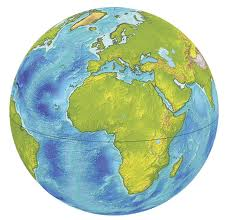
\includegraphics[scale = 0.5]{img/earth}
                \caption{Source image}
        \end{subfigure}
		\quad
        \begin{subfigure}[b]{0.3\textwidth}
                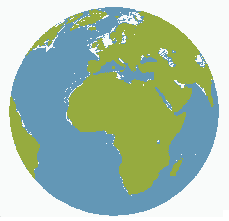
\includegraphics[scale = 0.5]{img/earth_segment}
                \caption{Segmented image}
        \end{subfigure}
		\caption{Example of segmenting an image. In this example the number of clusters specified is 3.}
		\label{fig:segmentation}
\end{figure}

\noindent \textbf{Background subtraction} \par
Background substraction (also known as foreground detection) is a process often used to detect moving objects with a static camera. The idea is that the background remains roughly the same in every image in a video stream, while moving objects enter and leaves the stream shortly after, or become part of the background after some time have passed. The rationale is to have a background image (or reference point) and then substract the image with the new object in it. Computing the difference will result in an image with only the moving object in it, that can be used for analysis. The absolute difference is computed almost like a standard \textit{matrix substraction} as shown in Equation \ref{eq:matrix_sub}. An example of background subtraction is shown in Figure \ref{fig:background_filtering}\\

\begin{equation}
\setlength{\arraycolsep}{5pt}
 \begin{bmatrix}
  a & b \\
  c & d \\
 \end{bmatrix} - 
 \setlength{\arraycolsep}{5pt} 
 \begin{bmatrix}
  e & f \\
  g & h \\
 \end{bmatrix} =
 \setlength{\arraycolsep}{5pt} 
 \begin{bmatrix}
  abs(a-e) & abs(b-f) \\
  abs(c-g) & abs(d-h) \\
 \end{bmatrix}
 \label{eq:matrix_sub}
\end{equation}

\begin{figure}
        \centering
        \begin{subfigure}[b]{0.3\textwidth}
                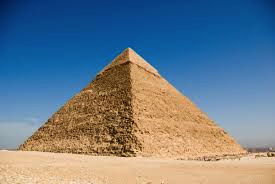
\includegraphics[scale = 0.35]{img/pyramid}
                \caption{Background image}
        \end{subfigure}
		\quad
        \begin{subfigure}[b]{0.3\textwidth}
                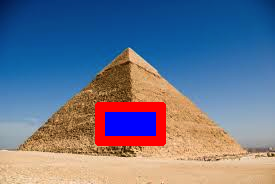
\includegraphics[scale = 0.35]{img/pyramid_new}
                \caption{Foreground image}
        \end{subfigure}
        \begin{subfigure}[b]{0.3\textwidth}
                
\includegraphics[scale = 0.35]{img/pyramid_object}
                \caption{Object detection}
        \end{subfigure}
		\caption{Example of detecting a new object on a static background. In this example all differences greater than zero is set to 255.}
		\label{fig:background_filtering}
\end{figure}

\newpage

\subsubsection{Framework} \mbox{}\par
\label{framework}
The theory behind computer vision techniques is solid. However to track an ant in an image solid theory and implementation is not enough. We have to keep in mind that this will have to be done on several consecutive images, without delaying the entire process, allowing the ant to escape the camera. Therefore effeciency is a key aspect as well. Chosing an effecient framework to help us track ants is therefore of outmost importance. OpenCV provides such a framework.\\

OpenCV is the shorthand for Open Computer Vision, and is an open source project started in 1999 and since maintained by Intel. It is written in C and C++ and runs on Linux, Windows and Mac OS X. OpenCV was designed from to beginning to be computationally efficient with a string focus on real-time applications. Another goal is to provide a simple-to-use computer vision infrastructure. Since its initial creation OpenCV has matured gradually, and along with it computer vision as well. Today OpenCV and computer vision is used in a broad context from web applications to survailance and aerial street maps.\\

Other computer vision frameworks exists but come short on several parameters. As stated in the requirements, tracking had to be done in \texttt{C}/\texttt{C++} which leaves out frameworks for higher level languages such as PyCVF for Python, imageJ for Java and OpenClooVision for C\#. Furthermore several frameworks exist that extends OpenCV or creates a simpler abstraction layer such as SimpleCV and other frameworks offers a very limited amount of features such as VisionBlocks. As a result OpenCV was chosen to be the framework of choice, both because of maturity and effeciency, but also because of the amount of computer vision features offered to its users.

\subsubsection{Realization} \mbox{}\par
Having presented several computer vision techniques and the framework used, this section will focus on applying these techniques in a real world scenario to find an actual ant within an image from a webcam. To be able to track the ant of interest and make it distinguishable from other ants, we will paint it with a color that is easier to detect than the ant itself. We want to track the ants on real ground material, and not just a static colored uniform background, and the ants available to us are either dark brown or black closely resembling the ground material found throughout Europe. It is therefore important to choose a color that is easy to detect on such material. For this reason we have chosen a white paint for testing purposes.\\

The image in Figure \ref{fig:ant} will be used as a reference point when showing how a certain computer vision technique performs in tracking the ant.

\begin{figure}[ht!]
  \centering
    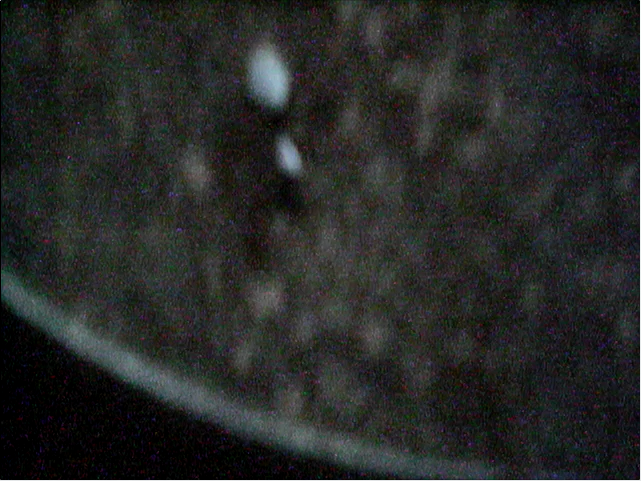
\includegraphics[scale=0.25]{img/ant.png}
  \caption{}
  \label{fig:ant}
\end{figure}


